\section{Implementation view}

I implementation view'et beskrives elementer som uden forklaring, ville være svære at forstå og bruge for udefrakommende. 

Indledningsvis beskrives de værktøjer der er benyttet til opsætning af dronens main controller, et arduino 2560 board. Dernæst beskrives værktøjer der er brugt til udvikling af server og webapplikation. Til sidst i afsnittet beskrives hvordan interne timere på arduino boardet er sat op til at genererer PWM signaler.  

\subsection{Opsætning af udviklings IDE til Arduino}

- Setup guide
- 


For at kunne anvende Atmel til projektet, skulle det først sættes op med de rigtige stier, clock indstillinger mm. Her blev der fulgt en guide \footnote{http://www.engblaze.com/tutorial-using-atmel-studio-6-with-arduino-projects/}, som trin for trin beskriver opsætningen af Atmel IDE'et. Guiden blev kun fulgt til og med \textit{"Build your project”}. 
For at kunne anvende Arduino biblioteker i Atmel kræver det at Arduino 1.0 eller højere er installeret. Det er muligt at tilføje eksterne biblioteker, ved at vælge Project i menuen og derefter vælge: "Add Existing Item", dette tilføjer et bibliotek til ens bibliotek. Derudover skal eksterne biblioteker også tilføjes compiler stien. Dette gøres ved at vælge Projects -> projektnavn properties. Her inde skal man vælge menuen ToolChain og ved Configurations vælge: All Configurations. Under menuen GNU C++ compiler vælges Directories, her inde skal man skrive stien for de eksterne biblioteker.

Megunolink er et program med en brugergrænseflade der kan anvendes til at sende og modtage seriel data fra en arduino.
For at kunne bruge megunolink sammen med Arduino kræver det at det bliver sat op på den rigtige måde.
Først hentes en gratis udgave af MegunoLink: MegunoLink Lite \footnote{http://www.megunolink.com/megunolink-lite/megunolink-lite-plotting-tool/}.

Efter installationen skal megunolink sættes op til at kunne compilere til en arduino.

\begin{enumerate}
	\item I configuration benyttes "use custom path" og ved AVRDude stien linkes til stien med AVRDude til arduino og configurationens stien. 
	\item I dropdown menuen vælges den arduino der skal bruges til projektet.
\end{enumerate}

\newpage

\begin{figure}[H]
	\centering
	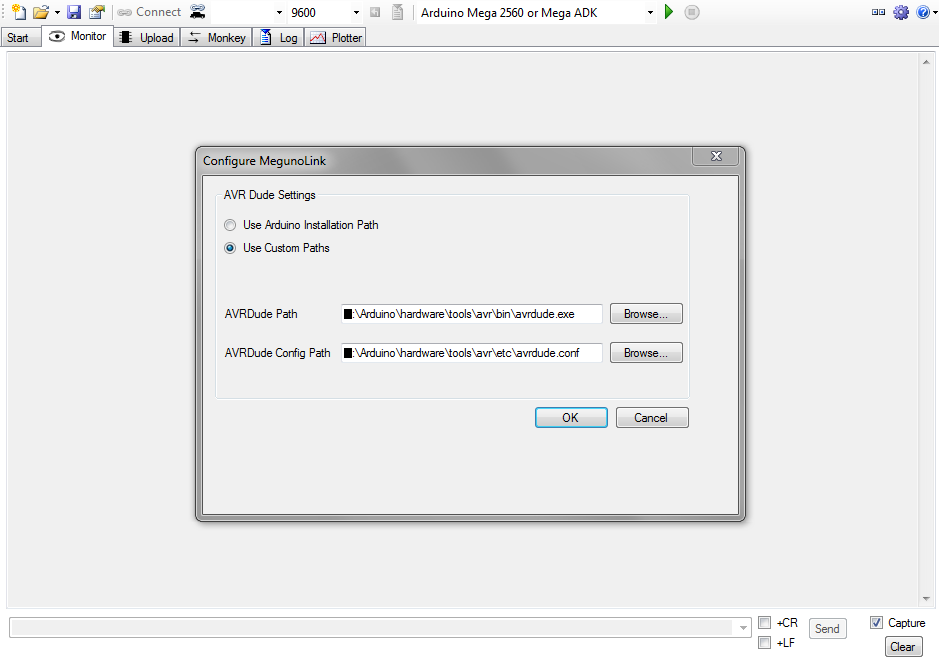
\includegraphics[width=0.85\textwidth]{Billeder/implementation/megunolink_config.png}
	\vspace{-.5cm}
	\caption{MegunoLink config}
	\label{fig:meglinkconf}
\end{figure}

For at kunne compilere, skal der linkes til projektets source fil. Hvis dette er udført korrekt, burde det være muligt at uploade source filen til arduino.

\subsection{Opsætning af eksterne bibliotekter til Atmel}

Når dronen henter informationer ned fra serveren, sker det med en karakter af gangen. Dette giver nogle vanskeligheder ifht. at skulle sortere i dataet der er modtaget. Når der hentes data, kan det bl.a. være længde- og breddegrader. Når det modtages, ved man ikke hvilken plads det ligger på i arrayet og hvilken størrelse værdierne har. Man kan, mellem server og drone, forud definere størrelserne der sendes/modtages, men det er hverken dynamisk eller præcis. Fra server siden er flyveopsætningen defineret som JSon objekter, hvilket er overskueligt og nem at sortere i. \\
I Atmel eller arduino findes der ikke et standard JSon bibliotek, der kan søge eller erstatte informationerne i et JSon objekt. Derfor har det været nødvendigt at finde et bibliotek der har kunnet tage denne type fil og bearbejde det som almindeligt data. Det anvendte bibliotek hedder aJson\footnote{https://github.com/interactive-matter/aJson} og er et frit tilgængeligt JSon bibliotek.Dette bibliotek er kombatibel med arduino. Ved hjælp af dette bibliotek, er det blevet muligt at hente flyveopsætningen fra serveren og afkode, oprette og ændre i dataet.

\newpage
\subsection{Opsætning af server}
Dette afsnit har til formål at beskrive hvordan et udviklingsmiljø sættes op på en givet maskine, så vider udvikling af systemet kan finde sted. Afsnittet forklarer også hvilke tredjeparts teknologier der er anvendt og eventuelle afhængigheder.

\subsubsection*{OS}
Det anbefales at udviklingen finder sted på en OS X eller Linux maskine, da UNIX-terminalen er et meget brugt værktøj og som standart er windows cmd meget "begrænset". Det kan dog lade sig gøre at bruge windows's cmd med nogle tweaks. Dette er ikke noget der vil blive forklaret yderligere og derfor er det kun UNIX-terminalen der er beskrevet i afsnittet.

\subsubsection*{IDE/Text Editor}
Da alt server opsætningen og logikken er skrevet i python, som er et højniveau script sprog, er der ikke nogle specielle krav til et IDE. Et simpelt tekst redigerings program er at fortrække. Det anbefales enten at bruge Sublime\footnote{http://www.sublimetext.com/2} Text Editoren eller Atom\footnote{https://atom.io/} Editoren. Begge text editors tilbyder god code highlightning og mulighed for at tilføje tredje parts pakker. Et udkast af de pakker der bruges er "PyLinter", "pep8" eller "Linter", som tjekker koden for evt. fejl i indentering, manglende kommentar eller kode standart.

\subsubsection*{Installation af software}
Dette underafsnit vil forklare hvordan diverse software pakker installeres på udviklingernes maskine og hvordan udviklerne starter den lokale server op. \\
Det første program der skal installeres er git. Skriv følgende i terminalen.

Linux:
\begin{lstlisting}[language=bash]
	$ sudo apt-get install Git
\end{lstlisting}

\textit{OS X: Kommer som standart med git installeret.}

Efter git er installeret på maskinen skal source koden klones fra github. Skriv følgende i terminalen.

\begin{lstlisting}[language=bash]
	$ git clone https://github.com/Opstrup/drone_backend
\end{lstlisting}

Efter source koden er hentet skal package manager programmet pip\footnote{https://pypi.python.org/pypi/pip} installeres. Skriv følgende i terminalen.

Linux:
\begin{lstlisting}[language=bash]
	$ sudo apt-get install python-pip
\end{lstlisting}

OS X:
\begin{lstlisting}[language=bash]
	$ sudo easy_install pip
\end{lstlisting}

Når pip er installeret skal scriptet "requirements.txt" køres, dette script ligger i roden af server projektet som blev hentet fra github. Skriv følgende i terminalen (da pip bliver brugt som package manager er kommandoen ens på Linux og OS X). \\

\begin{lstlisting}[language=bash]
	$ pip install -r requirements.txt
\end{lstlisting}

Efter scriptet er kørt og pip har installeret alle afhængigheder, er serveren klar til blive startet. For at starte serveren, skriv følgende i terminalen.

\begin{lstlisting}[language=bash]
	$ cd drone_backend_api/
	$ ./manage.py runserver
\end{lstlisting}


På figur \ref{fig:server_startup} ses et udklip af terminal vinduet ved server startup. Det ses at serveren er startet på "http://127.0.0.1:8000/", bemærk at denne url ikke bruges og vil derfor vise en: 404 error page not found fejl, hvis den tilgås. For at tilgå servere kan api endpoints, som beskrevet i Data view afsnittet, benyttes, http://127.0.0.1:8000/api/drones/.
\begin{figure}[H]
	\centering
	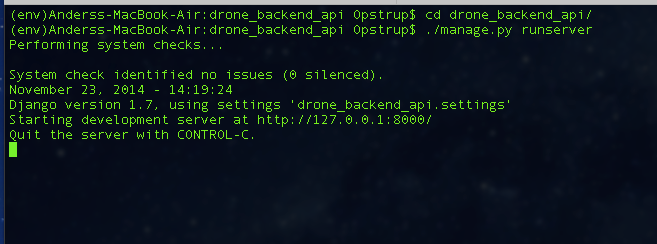
\includegraphics[width=0.85\textwidth]{Billeder/implementation/server_startup.png}
	\caption{Server startup msg}
	\label{fig:server_startup}
\end{figure}
\newpage

\subsubsection*{Mappestruktur}
Dette underafsnit vil forklare om den overordnede mappestruktur i projektet og giver en overordnet forståelse af django udvikling. \\

På figur \ref{fig:mappestruktur_1} ses den overordnet mappestruktur. I roden af mappen findes to væsentlige filer: db.sqlite3 hvilket er database filen til serveren, denne fil vil aldrig blive brugt direkte, men kun indirekte igennem django-frameworket. Den anden fil er manage.py, denne fil er main filen i hele projektet. Filen redigeres aldrig, men bruges kun via terminalen, til forskellige kommandoer på django-applikationen. \\

I roden findes der også to mapper "backend\_api" og "drone\_backend\_api". "drone\_backend\_api"  mappen er selve projekt mappen og "backend\_api" er applikations mappen.

\begin{figure}[H]
	\centering
	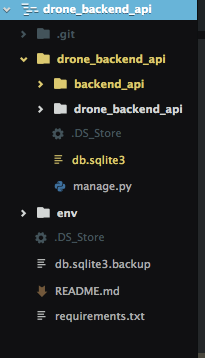
\includegraphics[width=0.2\textwidth]{Billeder/implementation/mappestruktur_1.png}
	\caption{Mappestruktur rod}
	\label{fig:mappestruktur_1}
\end{figure}

På figur \ref{fig:mappestruktur_2} ses projekt mappen, de væsentlige filer i denne mappe er settings.py og urls.py.
Settings.py er filen hvor alle tredje parts applikationer registeres i "INSTALLED\_APPS", filens sikkerhedsindstillinger  sættes op i "MIDDLEWARE\_CLASSES". 
Urls.py filen bruges til at registrere hvilke url's serveren kender og hvilke funktioner og views der skal præsenteres. Yderligere dokumentation omkring settings.py og urls.py kan findes under djangos egen dokumentation omkring settings\footnote{https://docs.djangoproject.com/en/dev/ref/settings/} og urls\footnote{https://docs.djangoproject.com/en/dev/ref/urls/}.

\begin{figure}[H]
	\centering
	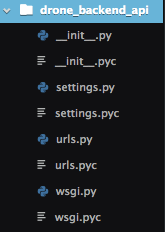
\includegraphics[width=0.2\textwidth]{Billeder/implementation/mappestruktur_2.png}
	\caption{Mappestruktur projekt mappe}
	\label{fig:mappestruktur_2}
\end{figure}

\newpage

På figur \ref{fig:mappestruktur_3} ses applikations mappen. Denne mappe indeholder alt logikken til serveren.

\begin{figure}[H]
	\centering
	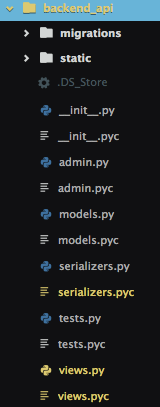
\includegraphics[width=0.2\textwidth]{Billeder/implementation/mappestruktur_3.png}
	\caption{Mappestruktur applikations mappe}
	\label{fig:mappestruktur_3}
\end{figure}

\textbf{admin.py} \\
Denne fil indeholder registrering af diverse tables i projektet. De kan tilgås via en admin page, hvor en administrator kan redigere i det data der ligger i databasen. Yderligere dokumentation omkring admin.py kan findes på\footnote{https://docs.djangoproject.com/en/dev/ref/contrib/admin/}.

\textbf{models.py} \\
Denne fil indeholder alt logikken til hvilke tabeller og attributter der eksistere i databasen. Via denne fil bliver db.sqlite3 filen som findes i roden, manipuleret. Yderligere dokumentation omkring models.py kan findes på\footnote{https://docs.djangoproject.com/en/dev/topics/db/models/}.

\textbf{serializers.py} \\
Denne fil indeholder serializers kaldes når et api-endpoint bliver kaldt. Via disse serializers finder serveren ud af hvilke data der skal hentes fra databasen og repræsenteres. Disse serializers bliver hovedsageligt brugt til at formatere dataen fra databasen til et JSON format. Yderligere dokumentation omkring serializers.py kan findes på\footnote{https://docs.djangoproject.com/en/dev/topics/serialization/}.

\textbf{views.py} \\
Denne fil håndtere de requests som kaldes og afgør ud fra dem hvilke serializer der skal generes og præsenteres. Yderligere dokumentation omkring views.py kan findes på\footnote{https://docs.djangoproject.com/en/dev/topics/class-based-views/}.
\newpage

\subsubsection*{Debug}
Dette underafsnit vil beskrive hvordan server software kan debugges og hvordan de forskellige værktøjer kan bruges.\\

\textbf{Terminal}\\
På figur \ref{fig:get_eksempel} ses et udklip af terminal vinduet, hvor to GET requests har fundet sted. Som det ses på billedet, er det muligt at debugge serveren og tjekke hvilke data sendes frem og tilbage ved hvert request. 

\begin{figure}[H]
	\centering
	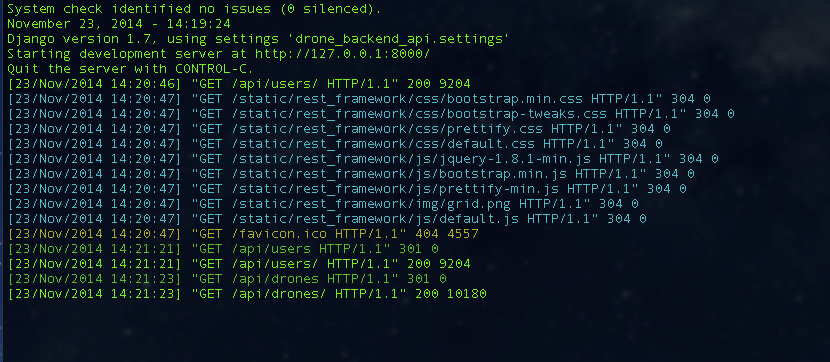
\includegraphics[width=1\textwidth]{Billeder/implementation/get_eksempel.png}
	\caption{GET eksempel}
	\label{fig:get_eksempel}
\end{figure}

\textbf{Browser}\\
På figur \ref{fig:browser_eksempel} ses et andet eksempel på hvordan browseren kan bruges til at debugge serveren. Her ses det hvilke data der kan hentes ved at gå til api-endpoint\\
"http://127.0.0.1:8000/api/drones/". Yderligere information kan findes under Data View afsnittet.

\begin{figure}[H]
	\centering
	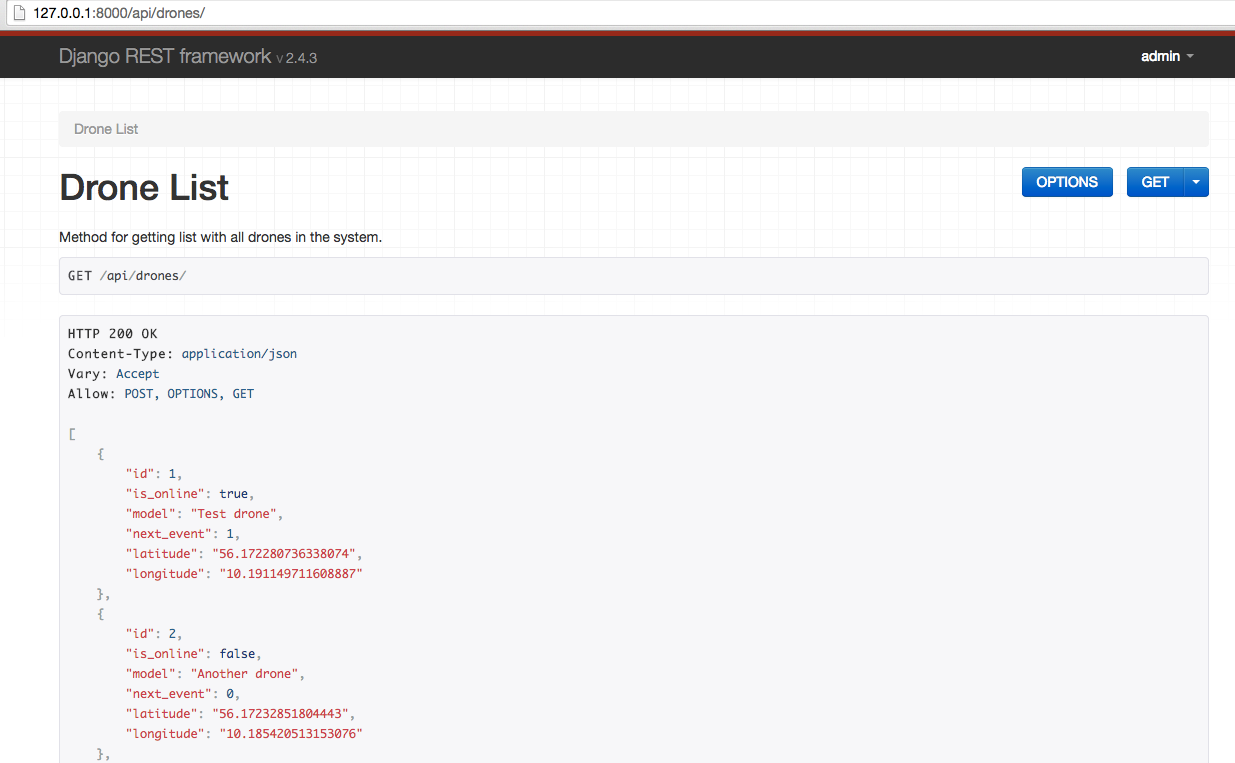
\includegraphics[width=1\textwidth]{Billeder/implementation/browser_eksempel.png}
	\caption{Browser eksempel}
	\label{fig:browser_eksempel}
\end{figure}

\vspace{1cm}

\subsubsection*{Tredje parts teknologier}
Til udviklingen af server softwaren er der benyttet nogle tredje parts teknologier, dette underafsnit beskriver hvilke og hvordan de er blevet brugt.

\textbf{Djangorestframework}\\
Django frameworket er et godt framework til udvikling af webapplikationer.Til projektet ønskes et RESTful api oven på django frameworket, derfor er der brugt et django-rest-frameworket\footnote{http://www.django-rest-framework.org/}. 

\textbf{django-cors-headers}\\
Cors headers\footnote{https://github.com/ottoyiu/django-cors-headers} er et django applikation som tilføjer CORS (Cross-Origin Resource Sharing) til applikationer. Dette gør det muligt at tilgå applikationen fra andre servere, som fx.  client softwaren som kan ligge på en anden server eller dronen som tilgår serveren udefra. 

\newpage

\newpage
\subsection{Opsætning webapplikation udvikling}
Dette afsnit har til formål at beskrive hvordan et udviklingsmiljø sættes op på en givet maskine så vider udvikling af systemet kan finde sted. Afsnittet forklare også hvilke tredjeparts teknologier der er anvendt og eventuelle afhængigheder.

For at kunne opsætte et udviklings miljø til client applikationen skal source koden først hente. Dette kan ske via git, skriv følgende kommando i terminalen.

\begin{lstlisting}[language=bash]
	$ git clone https://github.com/Opstrup/drone_frontend
\end{lstlisting}

\subsubsection*{Mappestruktur}
Dette underafsnit vil forklare om den overordnede mappe struktur i projektet og give en overordnet forståelse af angular client udvikling. \\

På figur \ref{fig:mappestruktur_client} ses mappestrukturen for client applikationen. Da Angular frameworket er opbygget over MVC\footnote{MVC model i forbindelse med Angular: https://docs.angularjs.org/guide/databinding} modellen er mappestrukturen opdelt så det afspejler denne model. I roden af projekt mappen findes to væsentlige file, app.js og index.html. app.js er settings filen for projektet, her bliver alle afhængigheder af projektet hentet ind og initialiseret, states i applikationen og dertilhørende controller bliver også registeret her\footnote{Information omkring app.js indstillingerne: https://docs.angularjs.org/guide/introduction}.\\
index.html er som kendt fra webudvikling den side som bliver hentet først ved et request, da Angular applikationer er et one paged app fungere det lidt specielt. Ved besøg af siden vil index side blive loaded samt javascript- og css-filer. Via Angular frameworket bliver alle andre sider så loaded ind i index siden, hvilket gøre applikationen meget hurtigt da filerne ikke skal indlæses igen.

\begin{figure}[H]
	\centering
	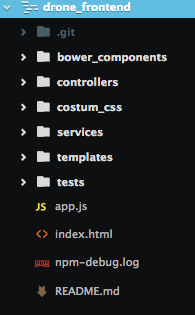
\includegraphics[width=0.2\textwidth]{Billeder/implementation/mappestruktur_client.png}
	\caption{Mappestruktur rod}
	\label{fig:mappestruktur_client}
\end{figure}

\textbf{bower\_components}\\
I denne mappe findes alle treide parts afhængigheder, i form af css og java script filer. Til håndtering af treide parts teknologier er der benyttet bower\footnote{http://bower.io/}, som er et package manager program til webudvikling.

\textbf{controllers}\\
I denne mappe findes alle controller\footnote{https://docs.angularjs.org/guide/controller} i systemet, som fungere på samme måde som kendt fra normal MVC.

\textbf{costum\_css}\\
Ud over bootstrap til håndtering af css'en, er der også blevet lavet nogle små filer med css kode. Disse filer findes i denne mappe.

\textbf{services}\\
I denne mappe findes alle services\footnote{https://docs.angularjs.org/guide/services} i systemet. Disse services indeholder alt buisness logikken i systemet og derved fungere som models i MVC modellen.

\textbf{templates}\\
I denne mappe findes alle html filerne for systemet, disser filer danner sammen med controllerne de views som bliver præsenteret i browseren\footnote{https://docs.angularjs.org/guide/templates}.

\subsubsection*{Udviklings miljø}
Opsætning af et udviklings miljø til client applikationen er rimelig simpel da source koden indeholder alt hvad der skal bruges for at kunne compile, der skal kun bruges en browser for at kunne starte applikationen. Til vider udvikling af applikationen vil det dog anbefales at der installeres nogle applikationer for at gøre udviklingen nemmere.

\textbf{Text editor}\\
Som alt andet web udvikling er det hele scripts som bliver kørt af browseren, derfor er der ingen specielle krav til et IDE af webudvikling. Nogle gode eksempler af text editor til web udvikling ville være Sublime eller Atom\footnote{Yderligere beskrevet i afsnittet om Server Opsætning}.

\textbf{Lokal web server}\\
For at applikationen fungere optimalt er det at anbefale at der installeres en web server på udviklerens maskine. Der er ikke nogle specielle krav til hvilke slags server. En simpel server kunne være en Apache server og for nem installation og opsætning kunne XAMPP\footnote{https://www.apachefriends.org/index.html} benyttes. Et andet eksempel på en web server kunne være en node.js server\footnote{http://nodejs.org/}. 

\textbf{Package management}\\
Som før nævnt er bower brugt til package management og det anbefales at der fortættes med dette da bower\footnote{http://bower.io/} selv downloader og installere de påkrævet filer, så udvikleren ikke skal tænke yderligere over dette.  

\newpage

\subsubsection*{Treide part teknologier}
Til udviklingen af web applikationen er der blevet brugt nogle treide parts teknologier, som er beskrevet yderligere i dette underafsnit.

\textbf{bootstrap}\\
Det populære bootstrap\footnote{http://getbootstrap.com/} css framework er benyttet til at give applikationen et flot design.

\textbf{ui-router}\\
Ui router\footnote{https://github.com/angular-ui/ui-router} er en applikation som er lavet til Angular frameworket som gør routing imellem div views meget simpel. 

\textbf{google-maps}\\
Google maps er blevet brugt til at vise kortet i applikationen og via google maps bliver der også hentet GPS-koordinater til de waypoints som dronen flyver efter. Google maps er ikke blevet benyttet som standart, men et angular applikation\footnote{https://angular-ui.github.io/angular-google-maps/} er blevet benyttet for at fungere bedre med den resterende kode.

\newpage
\section{Timer opsætning}

Da dronen skal flyve autonomt er det påkrævet at dronen skal styres via main controlleren (arduino boardet). Main controlleren styrer dronen ved at sende 6 forskellige pwm signaler til flight control boardet. De 6 pwm signaler bruges til at kontrollere og regulerer henholdsvis: Throttle, yaw, pitch, roll, alttitudehold og flightmode.

For at undgå at lave busywait når de forskellige pwm signaler skal ændres (skift i periodetid eller duty cycle) benyttes tre 16-bit timere som befinder sig på main controlleren. Arduino 2560 boardet har fire forskellige 16-bit timere, som hver kan styre pwm signal (output signal) på to digitale pins, hvis de  bruges korrekt. 

Fordelen ved at bruge timere til at kontrollere de 6 pwm signaler er primært, at pwm signalerne uafhængig og lynhurtigt kan ændres. For at ændre periodetid eller duty cycle på et pwm signal, skal værdien af et eller flere register blot skiftes. 

PWM signalets periodetiden kan forandres ved at ændre værdien af registeret der bruges til at bestemme hvor højt timeren skal ”tælle”, dette register kaldes typisk TOP eller ICRn. 
PWM signalets duty cycle kan forandres ved at ændre værdien af det register der bestemmer hvornår pwm signalet toggles. Dette register kaldes som regel \textit{Output compare}.

Det blev besluttet at bruge følgende tre timere i Fast PWM mode: \\
Timer1 - til kontrol af de to digitale pins 11 og 12.\\
Timer3 -  til kontrol af de to digitale pins 2 og 5.\\
Timer4 - til kontrol af de to digitale pins 6 og 7. \\

Figur \ref{fig:Timing_diagram} viser hvordan output kan se ud ved brug af en timer i Fast PWM mode.  

%kommentar
\begin{figure}[H]
	\centering
	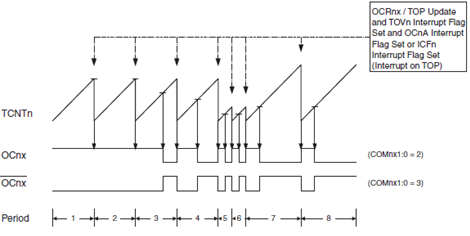
\includegraphics[width=1.\textwidth]{Billeder/Timer/0_timing_diagram.png}
	\caption{Fast PWM Mode, Timing Diagram}
	\label{fig:Timing_diagram}
\end{figure}

\newpage

I det følgende forklares hvordan de tre 16-bit timere er sat op. Bla. forklares valg at mode, udregning af frekvens, samt udregning af hvilke værdier der skal bruges i registerne ICRn og Output compare.

\subsection*{Mode 16-bit timer}

Når main controllerens 16-bits timere benyttes er det muligt at sætte timerne i 16 forskellige modes. Valget af mode styrer dels opløsningen af timeren, men styrer også hvordan timeren skal fungere. Timerne kan bruges i Normal mode, i CTC (Clear Timer on Compare), i Phase Correct PWM Mode eller i Fast PWM.

For at få den størst mulige opløsning benyttes de tre timerne i mode 14 - ”Fast PWM”. I mode 14 bestemmes værdien af TOP, af registeret ICRn som er et 16-bit stort register. Dette betyder at ICRn maksimalt kan sættes til værdien 0xFFFF (65535). 

%kommentar
\begin{figure}[H]
	\centering
	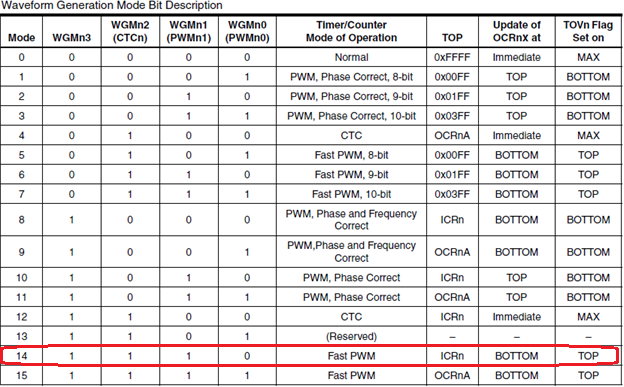
\includegraphics[width=1.\textwidth]{Billeder/Timer/1_mode.png}
	\caption{Fast PWM Mode, Timing Diagram}
	\label{fig:Timing_diagram}
\end{figure}

\newpage

\subsection*{Compare Output Mode}
Når det overordnede mode er valgt for timerne, skal compare output mode vælges. Compare output mode bestemmer hvornår PMW signalet på de forskellige pin sættes helholdvis højt og lavt.

Det besluttes at sætte Compare output mode til:  COMnA1 = 1 og COMnA0 = 0.  Med denne indstilling sættes PWM signalet lavt når timerens counter er lig OCnA eller OCnB og sættes højt igen hver gang timerens counter er lig 0. Indstillingerne sættes på samme vis for COMnB og COMnC.

%kommentar
\begin{figure}[H]
	\centering
	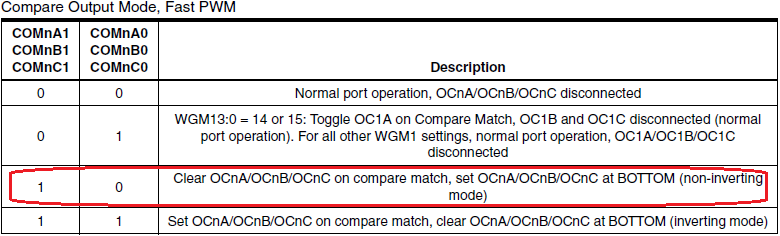
\includegraphics[width=1.\textwidth]{Billeder/Timer/2_compare_output_mode.png}
	\caption{Fast PWM Mode, Timing Diagram}
	\label{fig:Timing_diagram}
\end{figure}

 

\subsection*{TCCR3A}
Da både mode til 16-bit timeren og compare output er valgt kan registeret TCCR3A indstilles. Fra indstilling af mode til 16-bit timeren vides det at WGMn1 = 1, mens WGMn0 = 0. Yderlige vides det at COMnA1 = 1 og COMnA0 = 0 og at COMnB og COMnC skal se ligeledes ud.

Binært skal TCCR3A registeret se således ud: 0b10101010, hvilket i hex svarer til: 0xAA. 

Bemærk: Dette delafsnit tager udgangspunkt i TCCR3A registeret tilhørende timer 3.  TCCR1A og TCCR4A indstilles på samme vis.

%kommentar
\begin{figure}[H]
	\centering
	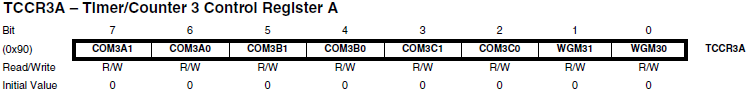
\includegraphics[width=1.\textwidth]{Billeder/Timer/3_TCCT3A.png}
	\caption{Fast PWM Mode, Timing Diagram}
	\label{fig:Timing_diagram}
\end{figure}

\newpage

\subsection*{Clock select}
Hvilken prescale der vælges har betydning for hvor hurtig en clock der bruges til timeren. I udgangspunkt er det en 16MHz clock der bruges, men ved at bruge prescale er det muligt at mindske clocken. Når der gøres brug af en 16-bit timer, har counteren maksimalt 65535 steps. 

Ud fra viden om clockens hastighed og antal steps i counteren kan frekvensen på timernes PWM signal udregnes således: Clock / antal steps = 244,14 Hz.  

Hvilket giver følgende periodetid: 1 / 244,14 Hz = 4,096 ms.

Sættes der prescale på clock’en vil frekvensen falde og periodetiden stige. Men da der ønskes periodetid så tæt på 2ms vælges det ikke at bruge prescale. 

%kommentar
\begin{figure}[H]
	\centering
	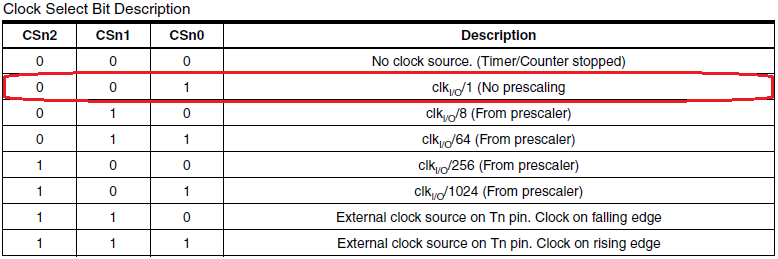
\includegraphics[width=1.\textwidth]{Billeder/Timer/4_CS.png}
	\caption{Fast PWM Mode, Timing Diagram}
	\label{fig:Timing_diagram}
\end{figure}
  

\subsection*{TCCR3B}
Da både mode til 16-bit timeren og clock select er valgt kan registeret TCCR3B indstilles. Fra indstilling af mode til 16-bit timeren vides det at WGMn3 = 1, mens WGMn2 = 1. Yderlige vides det at CSn2 = 0, CSn1 =0 og CSn0 = 1. 

Både ICNC3 (Input Capture Nolse Canceler) og ICES3 (Input Capture Edge Select) sættes lig 0.
Binært skal TCCR3B registeret se således ud: 0b00011001, hvilket i hex svarer til: 0x19. 

Bemærk: Dette delafsnit tager udgangspunkt i TCCR3B registeret tilhørende timer 3.  Registrene TCCR1B og TCCR4B tilhørende timer 1 og 4 indstilles på samme vis.

%kommentar
\begin{figure}[H]
	\centering
	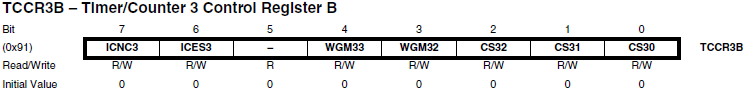
\includegraphics[width=1.\textwidth]{Billeder/Timer/5_TCCT3B.png}
	\caption{Fast PWM Mode, Timing Diagram}
	\label{fig:Timing_diagram}
\end{figure}


\subsection*{TCCR3C}
Force Output Compare A, B og C bruges kun når timeren er sat til et ikke PWM mode.  Derfor sættes Force Output Compare A, B og C = 0.
Binært skal TCCR3B registeret se således ud: 0b00000000, hvilket i hex svarer til: 0x00. 

Bemærk: Dette delafsnit tager udgangspunkt i TCCR3C registeret tilhørende timer 3.  Registrene TCCR1C og TCCR4C tilhørende timer 1 og 4 indstilles på samme vis.

%kommentar
\begin{figure}[H]
	\centering
	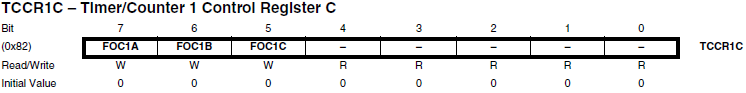
\includegraphics[width=1.\textwidth]{Billeder/Timer/6_TCCT3C.png}
	\caption{Fast PWM Mode, Timing Diagram}
	\label{fig:Timing_diagram}
\end{figure}
 

\subsection*{Indstilling Top og Compare match}
Reelt set er opsætningen af duty cycle og periodetid fuldstændig ligegyldigt. Det eneste der betyder noget, er at de PWM signaler der sendes til flight control boardet har pulsbredde mellem 1-2 ms.
 
Det vides at periodetiden på pwm signalerne vil være 4,096 ms når der arbejdes med clock på 16MHz, der ikke benyttes prescale og Top = 65535.

Ved opstilling af to simple ligninger, kan det beregnes hvilken værdi der skal skrives ind i compare match registeret for at skabe et pwm signal med pulsbredde på 1 ms.  

4,096 ms * x = 1 ms	Udtrykket omformes til: 	x = 1 ms / 4,096 ms = 0,244.

Værdi af Compare match for at opnå pulsbredde på 1ms:  Top * x = 65535 * 0,244 ~ 16000.

På samme vis kan det udregnes hvilken værdi der skal skrives i compare match for at få pulsbredde på 2 ms.

4,096 ms * x = 2 ms	Udtrykket omformes til: 	x = 2 ms / 4,096 ms = 0,488

Værdi af Compare match for at opnå pulsbredde på 1ms:  Top * x = 65535 * 0,488 ~ 32000.

Det er nu beregnet: Pulsbredde på 1ms fås ved compare match = 16000, mens pulsbredde på 2ms fås ved compare match = 32000. For at styre flight control board skal værdien i compare match altså veksle op og ned i størrelse mellem 16000 og 32000. 






